\documentclass[times,12pt]{article}
\usepackage{amsmath,amssymb,amsthm,mathrsfs,graphicx}
\usepackage{titlesec}
\usepackage{algorithm}
\usepackage{color}
\usepackage{float}
\usepackage{graphicx}
\usepackage{rotating}
\usepackage{url}
\usepackage{fancyhdr}

\pagenumbering{arabic}

\setlength{\parindent}{0pt}
\setlength{\parskip}{5pt plus 2pt minus 1 pt}

\topmargin  -15mm
\evensidemargin 0mm
\oddsidemargin  0mm
\textwidth  160mm
\textheight 235mm
\frenchspacing
\sloppy
\titlespacing{\section}{0pt}{\parskip}{0.01\parskip}
%%%%%%%%%%%%%%%%%%%%%%%%%%%%%%%%%%%%%%%%%%%%%%%%%%%%%%%%%%%%%%%%%%%%%%%

\begin {document}

\pagestyle{plain}

\begin{center}
{\fontsize{22}{20}\bf A Contact Detection Code using Triangles for Non-Spherical Particle Simulations\\
}\end{center}

\vspace{\fill}
\begin{center}\fontsize{16}{20}
\textbf{Konstantinos Krestenitis$^1$}\\
\today
\end{center}
\vspace{\fill}

\begin{center}
{\fontsize{10}{12}
}\end{center}

\begin{center}
$^1$School of Engineering and Computing Sciences, University of Durham, DH1 3LE, Durham\\
konstantinos.krestenitis@durham.ac.uk\\
Mechanics Research Group\\
\end{center}
\begin{center}
Supervised by\\
Dr Tobias Weinzierl\\
Dr Tomasz Koziara (former)\\
Professor Jon Trevelyan\\
\end{center}

\clearpage

\tableofcontents

\clearpage

\section{Introduction}
We present a Discrete Element Method (DEM) contact detection code that simulates rigid non-spherical particles on manycore shared memory machines and distributed memory computers. DEM is used to study granular particles in fields like soil mechanics. We rely on triangulated particle meshes to model surfaces. Spherical or multi-sphere models currently are state-of-the-art - due to a lack of well-suited software and runtime demands. Non-spherical particles promise to facilitate more accurate physics than sphere-based approaches \cite{AlonsoMarroqu2013}. The focus on triangles for rigid contact mechanics facilitates memory layouts allowing vectorised computation \cite{Alvarez2007, Koziara2005, Krestenitis2015}. It is vital to yield high performance on current and upcoming processor architectures to enable engineers to simulate more realistic materials.

It is important to investigate the problem of finding the minimum distance between triangles because of the changes in the computational hardware \cite{Dongarra2011}. The central processing unit architecture today and the future upcoming hardware support Single Instruction Multiple Data (SIMD)\cite{Alvarez2007} parallelism which allow data level parallelism. These speed-ups are enabled because of new instruction sets and wide vector register. Furthermore, shared memory parallelism at the node level as well as distributed memory for supercomputers can provide significant speed-ups. It is vital to extract resources available on current and upcoming hardware, the speed-ups enable more triangles to be used to describe surfaces. Consequently, our objective is to enable engineers to use an algorithm that is capable to handle the maximum amount of triangles per time step to do better engineering and science.

In the present work we propose a hybrid method that combines the advantages of two optimised triangle-to-triangle distance computation methods. It benefits from both performance and robustness of an iterative Newton-penalty and a brute force solver. We exploit shared memory parallelism and SIMD (Single Instruction Data) to perform contact detection at the node level. On distributed memory, we use spatial domain decomposition  whilst with the Message Passing Interface (MPI), we exploit asynchronous non-blocking communication to overlap data exchange with computation.

The state-of-the-art large scale DEM work, to the best of my knowledge, relies on sphere-based or multi-sphere particles \cite{Gonnet2013, Gonnet2014}. Large scale applications of spherical particles can be found in the field of molecular dynamics. Large scale non-spherical particle based DEM simulations in literature \cite{Girolami2012, Iglberger2009, Iglberger2010, Iglberger2011} often describe particles as convex polyhedra and contact detection is resolved with GJK (Gilbert-Johnson-Keerthi) \cite{Ericson2005} variants which require interpenetration and access to all vertices of the particle to detect contact on the surface. Interpenetration introduces contact point clustering and the problem of divergence \cite{Koziara2008, koziara2011, Krestenitis2015}. In addition, convex polyhedra based contact detection methods require undeterministic memory access to all particle simplices \cite{Ericson2005} which is contradictory to the aligned memory access imposed by SIMD for data locality. Triangle-based contact detection retain locality for vectorisation as well as increases accuracy of contact point generation \cite{Krestenitis2015}. Furthermore, the method can be extended to run on shared memory manycore and distributed memory machines.

The remainder of the paper is structured as follows. In Section 2, we describe the serial DEM  algorithm. In Section 3 we review two triangle-to-triangle distance algorithms. We create a new hybrid shared memory method that benefits from fast convergence and robustness. Next, in Section 3, we propose a distributed memory algorithm for contact detection that use asynchronous communication to overlap computation over communication. Section 4, discusses the future research directions.

\section{Algorithmic Overview}
\vspace{5mm}
\begin{itemize}
\item Completed since last report: Implemented serial DEM simulation with triangle-to-triangle contact detection using spring-dashpot contact forces, explicit time step.
\item New concepts: New shared memory hybrid method for computation of triangle-to-triangle distance.
\item Open questions: Best-case design of distributed memory implementation is not clear yet, real-world experiments are missing.
\end{itemize}

In contact mechanics, fluid-stucture interaction or other fields, it is an essential task to compute the distance between geometries to determine contact. Contact detection also is the most expensive algorithmic step \cite{Koziara2010, Wachs2012}. We present a Discrete Element Method (DEM) code that simulate particles that interact with spring-based contact. Non-spherical particles promise to facilitate more accurate physics than sphere-based approaches \cite{AlonsoMarroqu2013, Girolami2012}. The contact detection routine determines contact based on the distance between the triangles of every particle against all other. If two triangles are closer than a prescribed threshold, they are considered to contact each other. The use of triangles for rigid body contact dynamics rather than arbitrary polygons simplifies geometric checks and facilitates memory layouts that allow vectorised computation \cite{Eichenberger2004, Juurlink, Krestenitis2015, Krestenitis2016}.

The serial DEM Algorithm \ref{alg1} demonstrates the execution of contact detection, an O($n^2$) operation. In line 3 and line 4 the nested for loop indicate the complexity of iterating through all triangle pairs. In line 5 TTD(i, j) invokes a Triangle-to-Triangle Distance (TTD) algorithm that determines the distance between triangle i and triangle j. Based on the boundary layer margin contact model \cite{Krestenitis2015} to avoid penetration, we check if distance between Triangle i and j is smaller than a set margin (line 6). If the parent particle of triangle i and j is not the same then this indicate a contact point between the two particles (line 7). The contact point information at line 13 and line 14 is used to derive the forces. The forces accelerate the particles that are then integrated by an explicit time stepping scheme such as explicit Euler.

\clearpage

\begin{algorithm}	

1 \textbf{\textcolor{blue}{FOR}} time = 0; time $<$ simulation time; time+=step

2~~~//contact detection
		
3~~~~~~	\textbf{\textcolor{blue}{FOR}} i = 0 to N triangles

4~~~~~~~~~\textbf{\textcolor{blue}{FOR}} j = i+1 to N triangles
				
5~~~~~~~~~~~~distance = TTD(i,j)
				
6~~~~~~~~~~~~\textbf{\textcolor{blue}{IF}} (distance $<$ margin) AND ParticleID(i) != ParticleID(j)

7~~~~~~~~~~~~~~~contact(PID(i)).add(point, normal)

8~~~~~~~~~~~\textbf{\textcolor{blue}{ENDIF}}
			
9~~~~~~~~~\textbf{\textcolor{blue}{	ENDFOR}}
			
10~~~~~~\textbf{\textcolor{blue}{ENDFOR}}

11~~~//force derivation
		
12~~~~~~\textbf{\textcolor{blue}{FOR}} z = 0 to NB particles

13~~~~~~~~~	\textbf{\textcolor{blue}{FOR}} k = 0 to contacts(z).size()

14~~~~~~~~~~~~~~~force = granular(velocity(z), position(z), contacts(z).getcontact(k))

15~~~~~~~~~	\textbf{\textcolor{blue}{ENDFOR}}

16~~~~~~\textbf{\textcolor{blue}{ENDFOR}}
	
17~~~//explicit time stepping

18 \textbf{\textcolor{blue}{ENDFOR}}

\protect\caption{\label{alg1}DEM Serial Simulation Pseudo code}
\end{algorithm}


\begin{algorithm}	
  0 \textbf{\textcolor{blue}{FUNCTION}} force = penaltyForce(normal, relativeVelocity, depth, massA, massB)
  
  1~~mass = 1.0 / ((1/massA) + (1/massB));
  
  2~~velocitymagnitude = DOT(relativeVelocity, normal);
  
  3~~magnitude = SPRING*depth + DAMPER*sqrt(SPRING*mass)*velocitymagnitude;
  
  4~~force = magnitude*normal;
  
  5 \textbf{\textcolor{blue}{ENDFUNCTION}}
\protect\caption{\label{alg2}Spring-dashpot force algorithm}
\end{algorithm}

Algorithm \ref{alg2} shows the spring-based force derivation approach \cite{Koziara2008, solberg2000, Wachs2012, Williams1999}. To define contact points without penetration, we use the boundary layer margins to extend the surface boundary. Margin size is set based on velocities and time step size. When in contact, the margin overlap is used as the interpenetration depth. The contact point is at the middlepoint of the distance and normal direction is either side of the distance. At line 0, given the contact point normal, relative linear velocities, penetration depth and the mass of the two bodies we derive the interaction force to update the position of particle triangles on every time step.

\clearpage

\section{Vectorised Contact Detection}
\vspace{5mm}
\begin{itemize}
\item Completed since last report: Implemented serial and distributed memory robust contact detection and contact point generation.
\item New concepts: Created new hybrid algorithm for triangle-to-triangle distance calculation.
\item Open questions: Grain size and implications on shared memory load balancing.
\end{itemize}

We overview the brute force and penalty methods and we showcase the development of a new shared memory hybrid approach that benefits from both worlds. Both methods are implemented with two programming languages (MATLAB, C++). We focus on efficiency and we carefully benchmark the fragments on state-of-the-art architectures  with respect to run-time. We review two triangle-to-triangle distance algorithms, the brute force and the penalty method. The two methods form the basis of the hybrid method that we propose.


\subsection{Brute Force}
The brute force is the naive approach to contact detection, it computes all distances between geometrical primitives of the triangles. The method computes the distance between all line segments of one triangle with the line segments of the other using the segment-to-segment (Algorithm \ref{alg3}, line 22-30) distance function \cite{Ericson2005, Tropp2006}. Then for every point of one triangle it computes the distance against the other triangle using the point-to-triangle (Algorithm \ref{alg3}, line 3-8) function \cite{Eberly1999, Ericson2005}. The method requires evaluating the minimum distance among all comparisons performed to find the overall minimum distance in the end.

The algorithm is straight-forward because it relies on only two geometric comparisons. As seen in Algorithm \ref{alg3} in lines 3 to 21 the six comparisons yield one that defines the distance. For segment-to-segment, let $v_{1i}$, $e_{1i}$, $v_{2i}$, $e_{2i}$ be the vertices and edges of triangles $T_1$ and $T_2$. The brute force approach computes all fifteen distances $v_{1i}$-to-$T_2$, $v_{2i}$-to-$T_1$, $e_{1i}$-to-$e_{2i}$, and then we select the shortest distance. As seen in Algorithm \ref{alg3} in line 22 to 37 the algorithm determines the segment-to-segment distance between all segments of the triangle pair. Finally the algorithms finds the minimum of the two sets of comparisons to get the P and Q vertices that define the distance between two triangles. 

Optimization of the brute force method can at most rely on avoiding redundant evaluations parts of the computation. It is not possible to avoid logical branching because we have to evaluate all if statements to arrive to the solution. Therefore it is not possible to optimize the method for SIMD parallelism because of the branching. 

\begin{algorithm}
0~~\textbf{\textcolor{blue}{FUNCTION}} [min,P,Q] = \textbf{\textcolor{blue}{bf}}(A,B,C, D,E,F)

1~~T1=[A;B;C;];~~T2=[D;E;F;];

3~~[ptlist(1), P0(1,:)]= pt([D;E;F], T1(1,:));

4~~[ptlist(2), P0(2,:)]= pt([D;E;F], T1(2,:));

5~~[ptlist(3), P0(3,:)]= pt([D;E;F], T1(3,:));

6~~[ptlist(4), P0(4,:)]= pt([A;B;C], T2(1,:));

7~~[ptlist(5), P0(5,:)]= pt([A;B;C], T2(2,:));

8~~[ptlist(6), P0(6,:)]= pt([A;B;C], T2(3,:));

9~~ptmin = min(ptlist);

10~~\textbf{\textcolor{blue}{FOR}} i=1:6

11~~~~\textbf{\textcolor{blue}{IF}}(ptmin==ptlist(i))

12~~~~~~\textbf{\textcolor{blue}{IF}}(i<4)

13~~~~~~~~p1 = T1(i,:);~~p2 = P0(i,:);

15~~~~~~\textbf{\textcolor{blue}{ELSE}}

16~~~~~~~~p1 = P0(i,:);~~p2 = T2(i-3,:);

18~~~~~~\textbf{\textcolor{blue}{END;}}~~\textbf{\textcolor{blue}{break;}}

20~~~~\textbf{\textcolor{blue}{END;}}

21~~\textbf{\textcolor{blue}{END;}}

22~~[ss(1),sp1(1,:),sp2(1,:)]=segseg(T1(1,:),T1(2,:),T2(1,:),T2(2,:));

23~~[ss(2),sp1(2,:),sp2(2,:)]=segseg(T1(1,:),T1(2,:),T2(2,:),T2(3,:));

24~~[ss(3),sp1(3,:),sp2(3,:)]=segseg(T1(1,:),T1(2,:),T2(3,:),T2(1,:));

25~~[ss(4),sp1(4,:),sp2(4,:)]=segseg(T1(2,:),T1(3,:),T2(1,:),T2(2,:));

26~~[ss(5),sp1(5,:),sp2(5,:)]=segseg(T1(2,:),T1(3,:),T2(2,:),T2(3,:));

27~~[ss(6),sp1(6,:),sp2(6,:)]=segseg(T1(2,:),T1(3,:),T2(3,:),T2(1,:));

28~~[ss(7),sp1(7,:),sp2(7,:)]=segseg(T1(3,:),T1(1,:),T2(1,:),T2(2,:));

29~~[ss(8),sp1(8,:),sp2(8,:)]=segseg(T1(3,:),T1(1,:),T2(2,:),T2(3,:));

30~~[ss(9),sp1(9,:),sp2(9,:)]=segseg(T1(3,:),T1(1,:),T2(3,:),T2(1,:));

31~~ssmin = min(ss);

32~~\textbf{\textcolor{blue}{FOR}} i=1:9

33~~~~\textbf{\textcolor{blue}{IF}}(sslist(i) == ssmin)

34~~~~~~csp1 = sp1(i,:);~~csp2 = sp2(i,:);

36~~~~\textbf{\textcolor{blue}{END;}}

37~~\textbf{\textcolor{blue}{END;}}

38~~min = min(ssmin, ptmin);

39~~\textbf{\textcolor{blue}{IF}} min == ptmin

40~~~~P = p1;~~Q = p2;

41~~\textbf{\textcolor{blue}{ELSEIF}} min == ssmin

42~~~~P = csp1(:,:);~~Q = csp2(:,:);

43~~\textbf{\textcolor{blue}{END;}}
\protect\caption{\label{alg3}MATLAB Brute Force Solver.}
\end{algorithm}
\clearpage

\subsection{Penalty}

The second approach to solve the triangle-to-triangle  distance problem is by parameterising of the triangles such that the distance between them is formulated by a quadratic function and a solvable minimization problem. This approach is iterative compared to brute force. The method approximate the solution using Newton iterations.

The method relies on an optimization-based formulation of the distance between two points. Let $x$ and $y$ be two points, belonging respectively to triangle $T_1$ and $T_2$. Assuming that points $A, B, C$ are vertices of $T_1$ and that points $D, E, F$ are vertices of $T_2$, $x$ and $y$ can be defined using the following equations: 
\begin{align*}
T_{1}:x(a,b)=A+(B-A) \cdot a+(C-A)\cdot b
\end{align*}
\begin{align*}
T_{2}:y(g,d)=D+(E-D) \cdot g+(F-D) \cdot d
\end{align*} 
To find the minimum distance between $T_1$ and $T_2$ and the corresponding two closest points $P$, $Q$ on the two triangles we minimize
\begin{align*}
f\left(a,b,c,d\right)=\left\Vert x\left(a,b\right)-y\left(c,d\right)\right\Vert ^{2}
\end{align*} 

What has to be noted is that $x$ and $y$ have to stay within the area of the two triangles. The four parameters of the function $f$ have to comply with six inequality constraints:
\begin{align*}
min_{a,b,g,d} f(a,b,g,d)
\end{align*}  
$$such \:that: \: \{a\geq0,b\geq0, a+b\leq1, d\geq0, g\geq0, g+d\leq1 \}$$ 

\begin{figure}[!h]
\centering
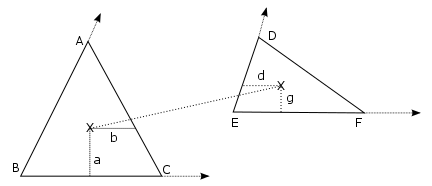
\includegraphics[width=0.6\textwidth]{c} \protect\caption{\label{fig1}Example of minimum distance and the corresponding barycentric points (parameters of objective function) on a pair of triangles in 3D. Triangle X:T1 has points A, B, C where barymetric parameters a,b correspond to point $x$ on the triangle. Triangle Y:T2 has points D,E,F where barymetric parameters g,d correspond to a point $x$. The two defined barymetric points define the minimum distance between the two triangles in 3D.}
\end{figure} 

To find the minimum of the parabolic constraint problem the Newton-Raphson method is used. Newton method use information from the curvature of the problem using the Hessian and gradient to arrive to a minimum point. To enforce the constraints the problem is transformed into a series of unconstrained problems with the augmentation of the objective function $f$ using the penalty-based method.

The penalty function penalizes the iteration so that the boundaries of the feasible region are valid; at least in a weak sense. Although there are factors that determine the number of iterations required the tuned-to-the-problem parameters yield a good number of Newton iterations that cannot be reduced to less than two; (initial guess to penalized boundary step, correction step).

\begin{figure}[!h]
\centering
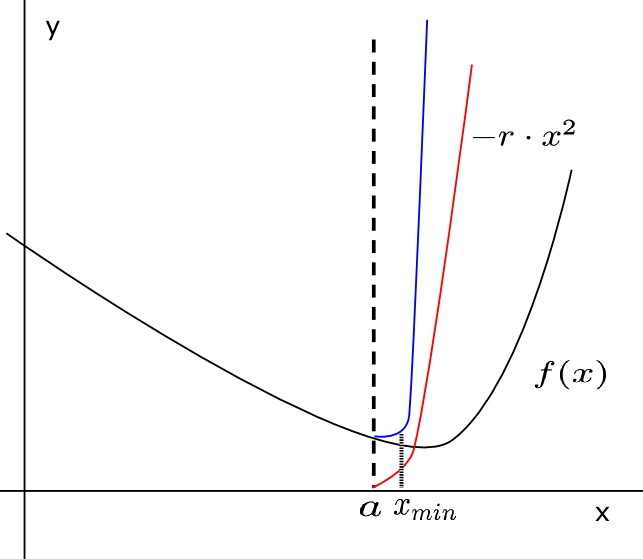
\includegraphics[width=0.5\textwidth]{penalty} \protect\caption{\label{fig2}Illustration of a 2D problem showing the penalty function (red line) penalizing the objective function (black line) f(x) under a constraint $a$ (dash line) to create the feasible region (blue line).}
\end{figure} 

This iterative approach adds a penalty term to the objective function to penalize the solution when outside of the feasible region: 
\begin{equation}\label{eq:penalty}
P(x)=f(x)+r\sum_{i=1...6}max(0,c(x_{i}))^{2}
\end{equation}
Where r is the penalty parameter (Figure \ref{fig2}). Newton iterations always converge to a solution slightly on the outside of the feasible region. Convergence can be controlled by the r penalty parameter that controls the sharpness of the curve for the constraints. One aspect that requires care however is the invertibility of the Hessian $\nabla\nabla P$. 

Furthermore that the problem is ill conditioned and a Quasi-Newton method has to be used. The Hessian matrix is not invertible so it is not possible to solve the direction of the search by computing the Hessian and gradient. This illustrates the fact that $f$ has multiple minima and $\nabla\nabla f$ is singular. Consequently, $\nabla\nabla P$ is also singular inside of the feasible region. The ill conditioning is caused by the problem definition itself, where there is a state where there are multiple solutions to the problem based on the orientation of the two triangles. This is also revealed by the two zero eigenvalues of the Hessian. Because of the ill-conditioning, we use a quasi-Newton approach, where the Hessian is approximated by a perturbed operator $\nabla\nabla P + \epsilon I$. $I$ is an identity matrix and $\epsilon$ is suitably small. 

\begin{algorithm}
0~~\textbf{\textcolor{blue}{FUNCTION}}~x~=~\textbf{penalty}(A,~B,~C,~D,~E,~F,~rho,~tol)

1~~BA~=~B-A;~CA~=~C-A;~ED~=~E-D;~FD~=~F-D;

2~~hf~=~{[}2{*}BA{*}BA',~2{*}CA{*}BA',-2{*}ED{*}BA',-2{*}FD{*}BA';

3~~~~~~~~2{*}BA{*}CA',~2{*}CA{*}CA',-2{*}ED{*}CA',-2{*}FD{*}CA';

4~~~~~~~-2{*}BA{*}ED',-2{*}CA{*}ED',~2{*}ED{*}ED',~2{*}FD{*}ED';

5~~~~~~~-2{*}BA{*}FD',-2{*}CA{*}FD',~2{*}ED{*}FD',~2{*}FD{*}FD'{]};

6~~x~=~{[}0.33;~0.33;~0.33;~0.33{]};

3~~\textbf{\textcolor{blue}{FOR}}~i=1:99

4~~~~X~=~A+BA{*}x(1)~+~CA{*}x(2);

5~~~~Y~=~D+ED{*}x(3)~+~FD{*}x(4);

6~~~~gf~=~{[}2{*}(X-Y){*}BA';~2{*}(X-Y){*}CA';~-2{*}(X-Y){*}ED';~-2{*}(X-Y){*}FD'{]};~

7~~~~h~=~{[}-x(1);~-x(2);~x(1)+x(2)-1;~-x(3);~-x(4);~x(3)+x(4)-1{]};

8~~~~dh~=~{[}-1,~0,~1,~0,~0,~0;~0,~-1,~1,~0,~0,~0;

9~~~~~~~~~~~0,~0,~0,~-1,~0,~1;~0,~0,~0,~0,~-1,~1{]};

10~~~mask~=~h'~$>$=~0;

11~~~dmax~=~dh.{*}~{[}mask;~mask;~mask;~mask{]};

12~~~gra~=~gf~+~rho~{*}~dmax~{*}~max(0,h(:));

17~~~hes~=~hf~+~rho{*}dmax{*}dmax'~+~eye(4,4)/rho\textasciicircum{}2;

18~~~dx~=~hes\textbackslash{}gra;

19~~~DX~=~BA{*}dx(1)~+~CA{*}dx(2);

20~~~DY~=~ED{*}dx(3)~+~FD{*}dx(4);

21~~~error~=~sqrt(DX{*}DX'+DY{*}DY');

22~~~\textbf{\textcolor{blue}{IF}}~error~$<$~tol,~\textbf{\textcolor{blue}{BREAK}};~\textbf{\textcolor{blue}{END}}

23~~~x~=~x~-~dx;

24~\textbf{\textcolor{blue}{END}}

25~\textbf{\textcolor{blue}{END}}
\protect\caption{\label{alg4}MATLAB Penalty Solver.}
\end{algorithm}

The penalty algorithm in pseudocode language is shown in Algorithm \ref{alg4}. It accepts A, B, C, D, E, F vector coordinates for triangle T1(A, B, C), T2(D, E, F) as well as the required parameters for the algorithm to be solved. Rho is the penalty parameter that controls the steepness of the P(x) function (equation \ref{eq:penalty}) , eps is the perturbation parameter for the hessian matrix of the problem along its diagonal to make the matrix solvable. Tol is the tolerance for convergence (Floating point accuracy). In line 6 of Algorithm \ref{alg4} an initial guess is chosen to be the center of the two triangles, then the for loop initiates the Newton iterations to find the points on the X, Y triangle planes under the constraints c. For each of the six constraints (line 12) the max function of the penalty is determined so that every possible active constraint is detected. In line 19 and line 20 the gradient and Hessian of P Penalty function is evaluated to be provided to the Gaussian elimination direct solver so that a Newton direction DX is solved. If the Newton step is large enough over the specified tolerance then the iteration is converged else the direction is used and the loop is executed once more recursively.

The penalty method is well-suited for SIMD optimisation. We can concurrently determine the distance between multiple triangle pairs as long as we use the same number of Newton steps: Up to four or eight
triangle pair distances then are determined at the same time. Such a speed-up statement however has to be read carefully. While the concurrency is high, it is not clear a priori how many Newton steps are
required. A high number of Newton steps can render the penalty method slower than a brute force approach.

\subsection{Hybrid}
We propose a new hybrid algorithm that combines both penalty and brute force to solve the distance problem $f\left(a,b,c,d\right)_{min}=\left\Vert x\left(a,b\right)-y\left(c,d\right)\right\Vert ^{2}$. The method benefits both from iterative penalty-based approximation performance and brute force robustness. The algorithm switches from penalty to brute force on run-time when there is no convergence. In a modern CPU environment the hybrid method exploits the Simultaneous Multi-Threading (SMT) microprocessor architecture on top of Single Instruction Multiple Data (SIMD) parallelism \cite{Gonnet2014}.

We exploit the multi-threaded environment by splitting the computational workload into groups of batches. The batches are a set of triangle pairs that are selected sequentially in a memory aligned vector array. We fuse triangle comparisons with threads to exploit thread level parallelism and wide SIMD registers. Convergence checking is performed on a per-batch basis to determine fall-back to brute force. 

\begin{figure}[!h]
\centering
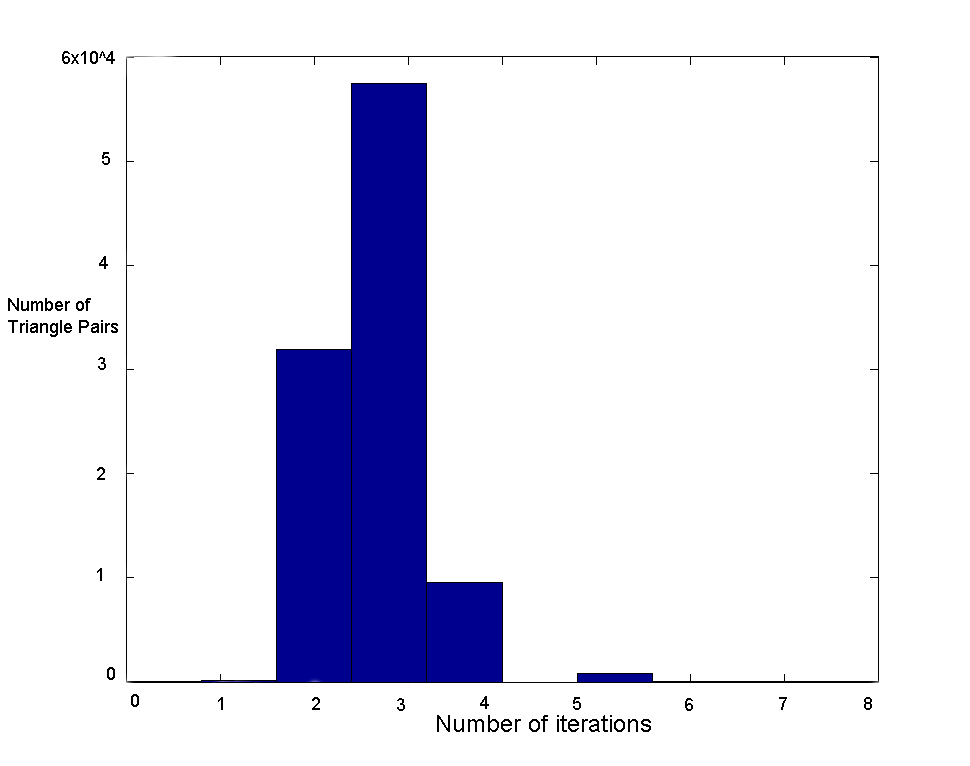
\includegraphics[width=0.8\textwidth]{hist} \protect\caption{\label{fig3}Histogram of iterations required to solve random pairs of triangles using penalty.}
\end{figure}

Based on empirical studies and tuning of the penalty parameter and the regularization variable, the majority of triangle pairs are solved within four iterations as shown in Figure \ref{fig3}. When the batch is solved within four iterations then it runs a penalty solver but that is not always the case. The memory distribution of pairs of triangles that do not converge within four Newton iterations are not known a priori because the solution depends on the underlying geometry. Triangle pairs that do not converge skew the error margin of the batch creating the worse case scenario where the hybrid method becomes a brute force solver. It is not possible to predict the sparse distribution of non-convergent triangle pairs during run-time.

A tuning factor is the batch/grain size. The grain size is the computation assigned per thread in terms of number of vectorized triangle pairs. The grain size affects the error value and the SIMD performance performed by penalty and brute force. The larger the grain the more triangle comparisons can be fused into SIMD statements. However, if one or more triangle fail convergence, the whole batch may need to fall back to brute force. The grain size affects thread-level load balancing. in theory, dynamic scheduling should resolve imbalances. Dynamic scheduling uses the work queue to provide a dynamically sized block of loop iterations to each thread during run-time. This method creates an extra scheduling overhead to the algorithm, due to thread safety and other load balance auxiliary metrics. Experiments show that dynamic balancing does not yield performance improvement due to overhead. Static scheduling is sufficient. Tuning the grain is non-trivial due to the random distribution of triangle pairs in memory. Trial and error fine-tuning over a given set of random triangles work best for static load balancing. The batch size for random triangles is optimal at size eight.

\clearpage

\begin{algorithm}	

1~~~n=sizeoftriangles      

2~~~batchSize = 4;

3~~~error[batchSize]

4~~~batchError = 0.0;

5~~~\textbf{\textcolor{blue}{FOR}} (k=0; k$<$n/batchSize; k++) //grain-size is four

6~~~~~~~batchError = 0.0;

7~~~~~~\textbf{\textcolor{blue}{PRAGMA OMP PARALLEL FOR SIMD REDUCTION (+:batchError)}}

8~~~~~~\textbf{\textcolor{blue}{FOR}} (l=0; l$<$batchSize; l++) 

9~~~~~~~~i=k*batchSize + l;

10~~~~~~~~distance[i] = penalty(T1[i], T2[i], P[i], Q[i], error[l]);

11~~~~~~\textbf{\textcolor{blue}{ENDFOR}}

12~~~~~~batchError = 0.0;

13~~~~~~\textbf{\textcolor{blue}{FOR}} (l=0; l$<$batchSize; l++) 

14~~~~~~~~~batchError += error[l];

15~~~~~~\textbf{\textcolor{blue}{ENDFOR}}

16~~~~~~\textbf{\textcolor{blue}{IF}}(batchError/batchSize$>$1E-8)

17~~~~~~~~~\textbf{\textcolor{blue}{PRAGMA OMP PARALLEL FOR SIMD}}

18~~~~~~~~~\textbf{\textcolor{blue}{FOR}} (l=0; l$<$batchSize; l++)

19~~~~~~~~~~~~i = k*batchSize + l;

20~~~~~~~~~~~~distance[i] = bf(T1[i], T2[i], P[i],Q[i]);

21~~~~~~~~~\textbf{\textcolor{blue}{ENDFOR}}

22~~~~~~\textbf{\textcolor{blue}{ENDIF}}

23~~~\textbf{\textcolor{blue}{ENFOR}}

\protect\caption{\label{alg5}Hybrid Contact Detection}
\end{algorithm}

In Algorithm \ref{alg5} we show the serial pseudocode of the hybrid penalty-brute force method. In line 2 we set the batchSize to four, that is the grain size. In line 6 we split the computational workload n into batches based on the grain size and loop through the batches. In line 9 we initiate a parallel threaded loop over SIMD operations within each batch and solve each triangle pair with penalty. Line 9 specifies the reduction instruction to perform a parallel sum reduction on the batch error per pair. In line 10 the penalty method is executed for one triangle pair T1[i] and T2[i] where P[i], P[i] are vertex points that define the three dimensional distance[i]. In line 14 the overall batch error is summed and in line 16 it is compared against a manually set tolerance. If batchError exceeds the tolerance then the algorithm calls brute force.

We implemented the new hybrid method in the C programming language with SIMD enabled on Intel Sandy Bridge 2.0GHz i5.  In Figure \ref{fig4} we showcase the measurements of shared memory hybrid approach against the penalty and brute force methods. As expected the hybrid performance is settled between brute force and penalty. The method is slower than penalty because there are batches of triangle pairs that do not reach  the convergence tolerance. It is faster than brute force because no significant number of batches fail the tolerance. The hybrid algorithm scales over the second socket of the CPU but does not gain significant performance between eight and sixteen cores because of data stagnation at the socket interconnect. Theoretically, performance can be tuned further by investigating the load balancing implications on the non-deterministic element of the algorithm. The results are sufficient with static scheduling for proof of concept.

\begin{figure}[!h]
\centering
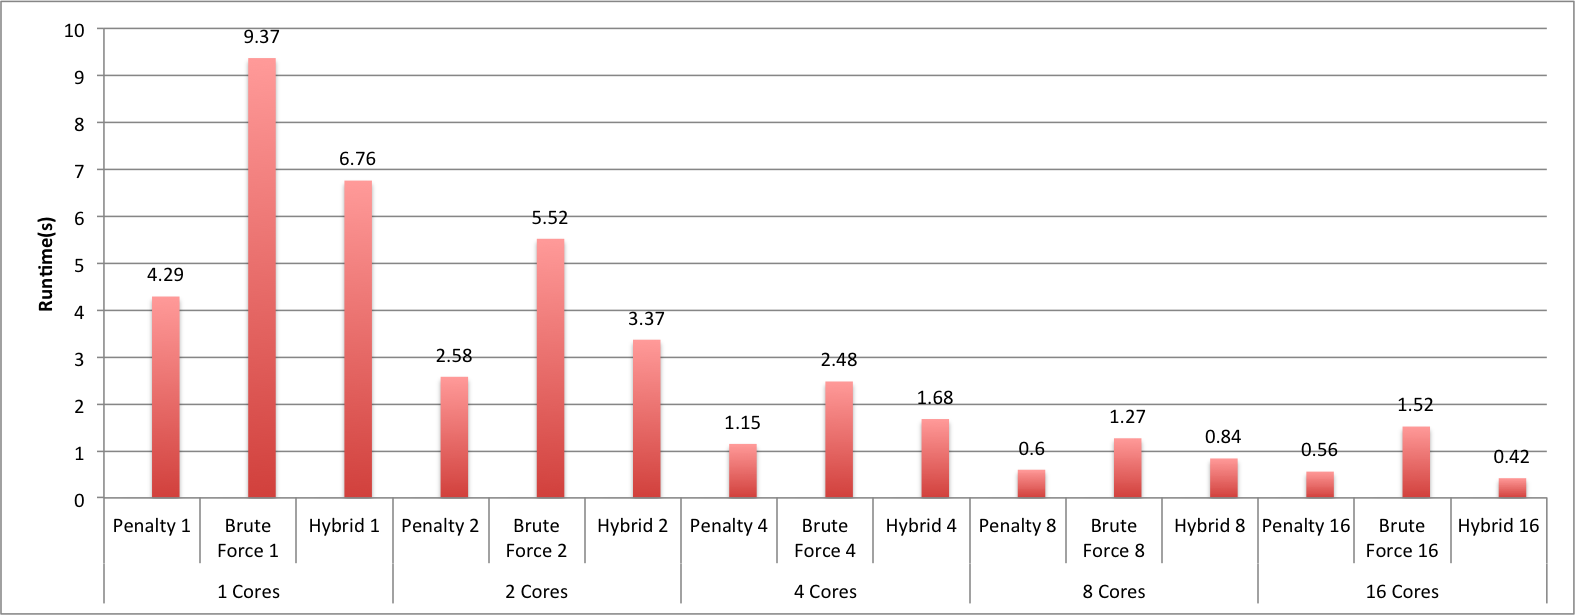
\includegraphics[width=1\textwidth]{hybrid} \protect\caption{\label{fig4}Run-time comparison of the penalty, brute force and the hybrid method over no of cores.}
\end{figure}

\section{Domain Decomposition for Contact Detection}
\vspace{5mm}
\begin{itemize}
\item Completed since last report: Implemented domain decomposition for distributed memory load balancing using library, MPI blocking communication for data migration. 
\item New concepts: Overlapping process communication for contact detection with ghost data. Asynchronous communication waiting
time significant as number of ranks increase.
\item Open questions: multilayer grid/spacetree implementation for DEM 
\end{itemize}

We further scale the computation of triangle-to-triangle contact with the Message Passing Interface (MPI) \cite{Forum:1994:MMI:898758} for distributed memory computation. Our DEM-based contact detection is inspired by molecular dynamics simulations, where millions of spheres are simulated. State-of-the-art MD computation is decomposed into smaller computational sub-domains and communication exchanges necessary boundary information. Similar computational stages are applied by us in the DEM-based contact detection algorithm. We study synchronous and asynchronous modes of data exchange and how two communication strategies can be exploited to increase performance and minimize computation.

The distributed memory DEM contact detection algorithm is performed in three stages. In stage one the computational domain is divided into equally balanced sub-domains. In stage two, data migration assigns the sub-domains to MPI instances. In stage three, we compute the distances to determine contact between all triangles. In stage four we accumulate the forces and in stage five we perform the explicit time step integration.

\subsection{Domain Decomposition}

To scale the performance of contact detection simulation, the computational workload has to be processed in parallel by splitting the domain into sub-domains and computation deployment is based on it, making the decomposition an important stage. Decomposition affects load balancing and the communication patterns of the simulation. Communication is essential when sub-domains are inter-dependent since new boundaries are introduced with decomposition. It is important to decompose evenly whilst also reducing sub-domain communication. There are three types of decomposition that are widely used in different contexts \cite{Eckhardt2014, Plimpton1995} that can apply in DEM. Decomposition by particle, decomposition by force and spatial decomposition. 

In domain decomposition by particle \cite{koziara2011}, the domain is divided such that all sub-domains hold equal number of particles. For N particles we split the domain to N parts and we assign them to P processors (N/P). The sub-domain boundary is always located at the space between particles. In this method an all-to-all communication is required to detect contact points because they are always located at the sub-domain boundary. The global communication is a major disadvantage for small particles as each processor communicates with all other processors, staggering the overall parallel processing. Another disadvantage is the non-equal splitting (N/P) as some particles may require more computation than others (i.e. more triangles). The main advantage of particle-based decomposition is the implementation simplicity \cite{Plimpton1995}.

An alternative decomposition approach found in literature is force-based decomposition that is often applied in molecular dynamics (MD) and smoother particle hydrodynamic (SPH) simulations \cite{Bowers2007, Gaburov, Gonnet2014, Plimpton1995, Rycroft2012, Shaw2005}. The method formulates a interaction force matrix that solves the contact detection and the forces as a group of linear equations. The matrix is decomposed into small blocks and shared on each process to solve in parallel. Force based decomposition assume short-range interactions and thus a dense force matrix to solve. In force based methods, the advantage is that computation is decomposed without any spatial information from the particles. The major disadvantage in DEM applications is the assumption of dense and uniform sparse force matrices, the assumption can be wrong leading to imbalanced domains on run-time.   

According to N-body simulation literature \cite{Eckhardt2014, Fleissner, Wachs2012a, zomorodian2002} the state-of-the-art method for supercomputing applications is the spatial decomposition. Our decomposition is based on the spatial position of vertices using Recursive Coordinate Bisection (RCB) \cite{ZoltanIsorropiaOverview2012}. In RCB, the computational domain is first divided into two regions by a cutting plane orthogonal to one of the coordinate axes so that half the work load is in each of the sub-regions. The splitting direction is determined by computing in which coordinate direction the set of objects is most elongated, based upon the geometric locations of the objects. Each triangle vertex thus is owned and persistently stored exclusively on one process/sub-domain for the whole duration of the timestep. 

\begin{figure}[!h]
\centering
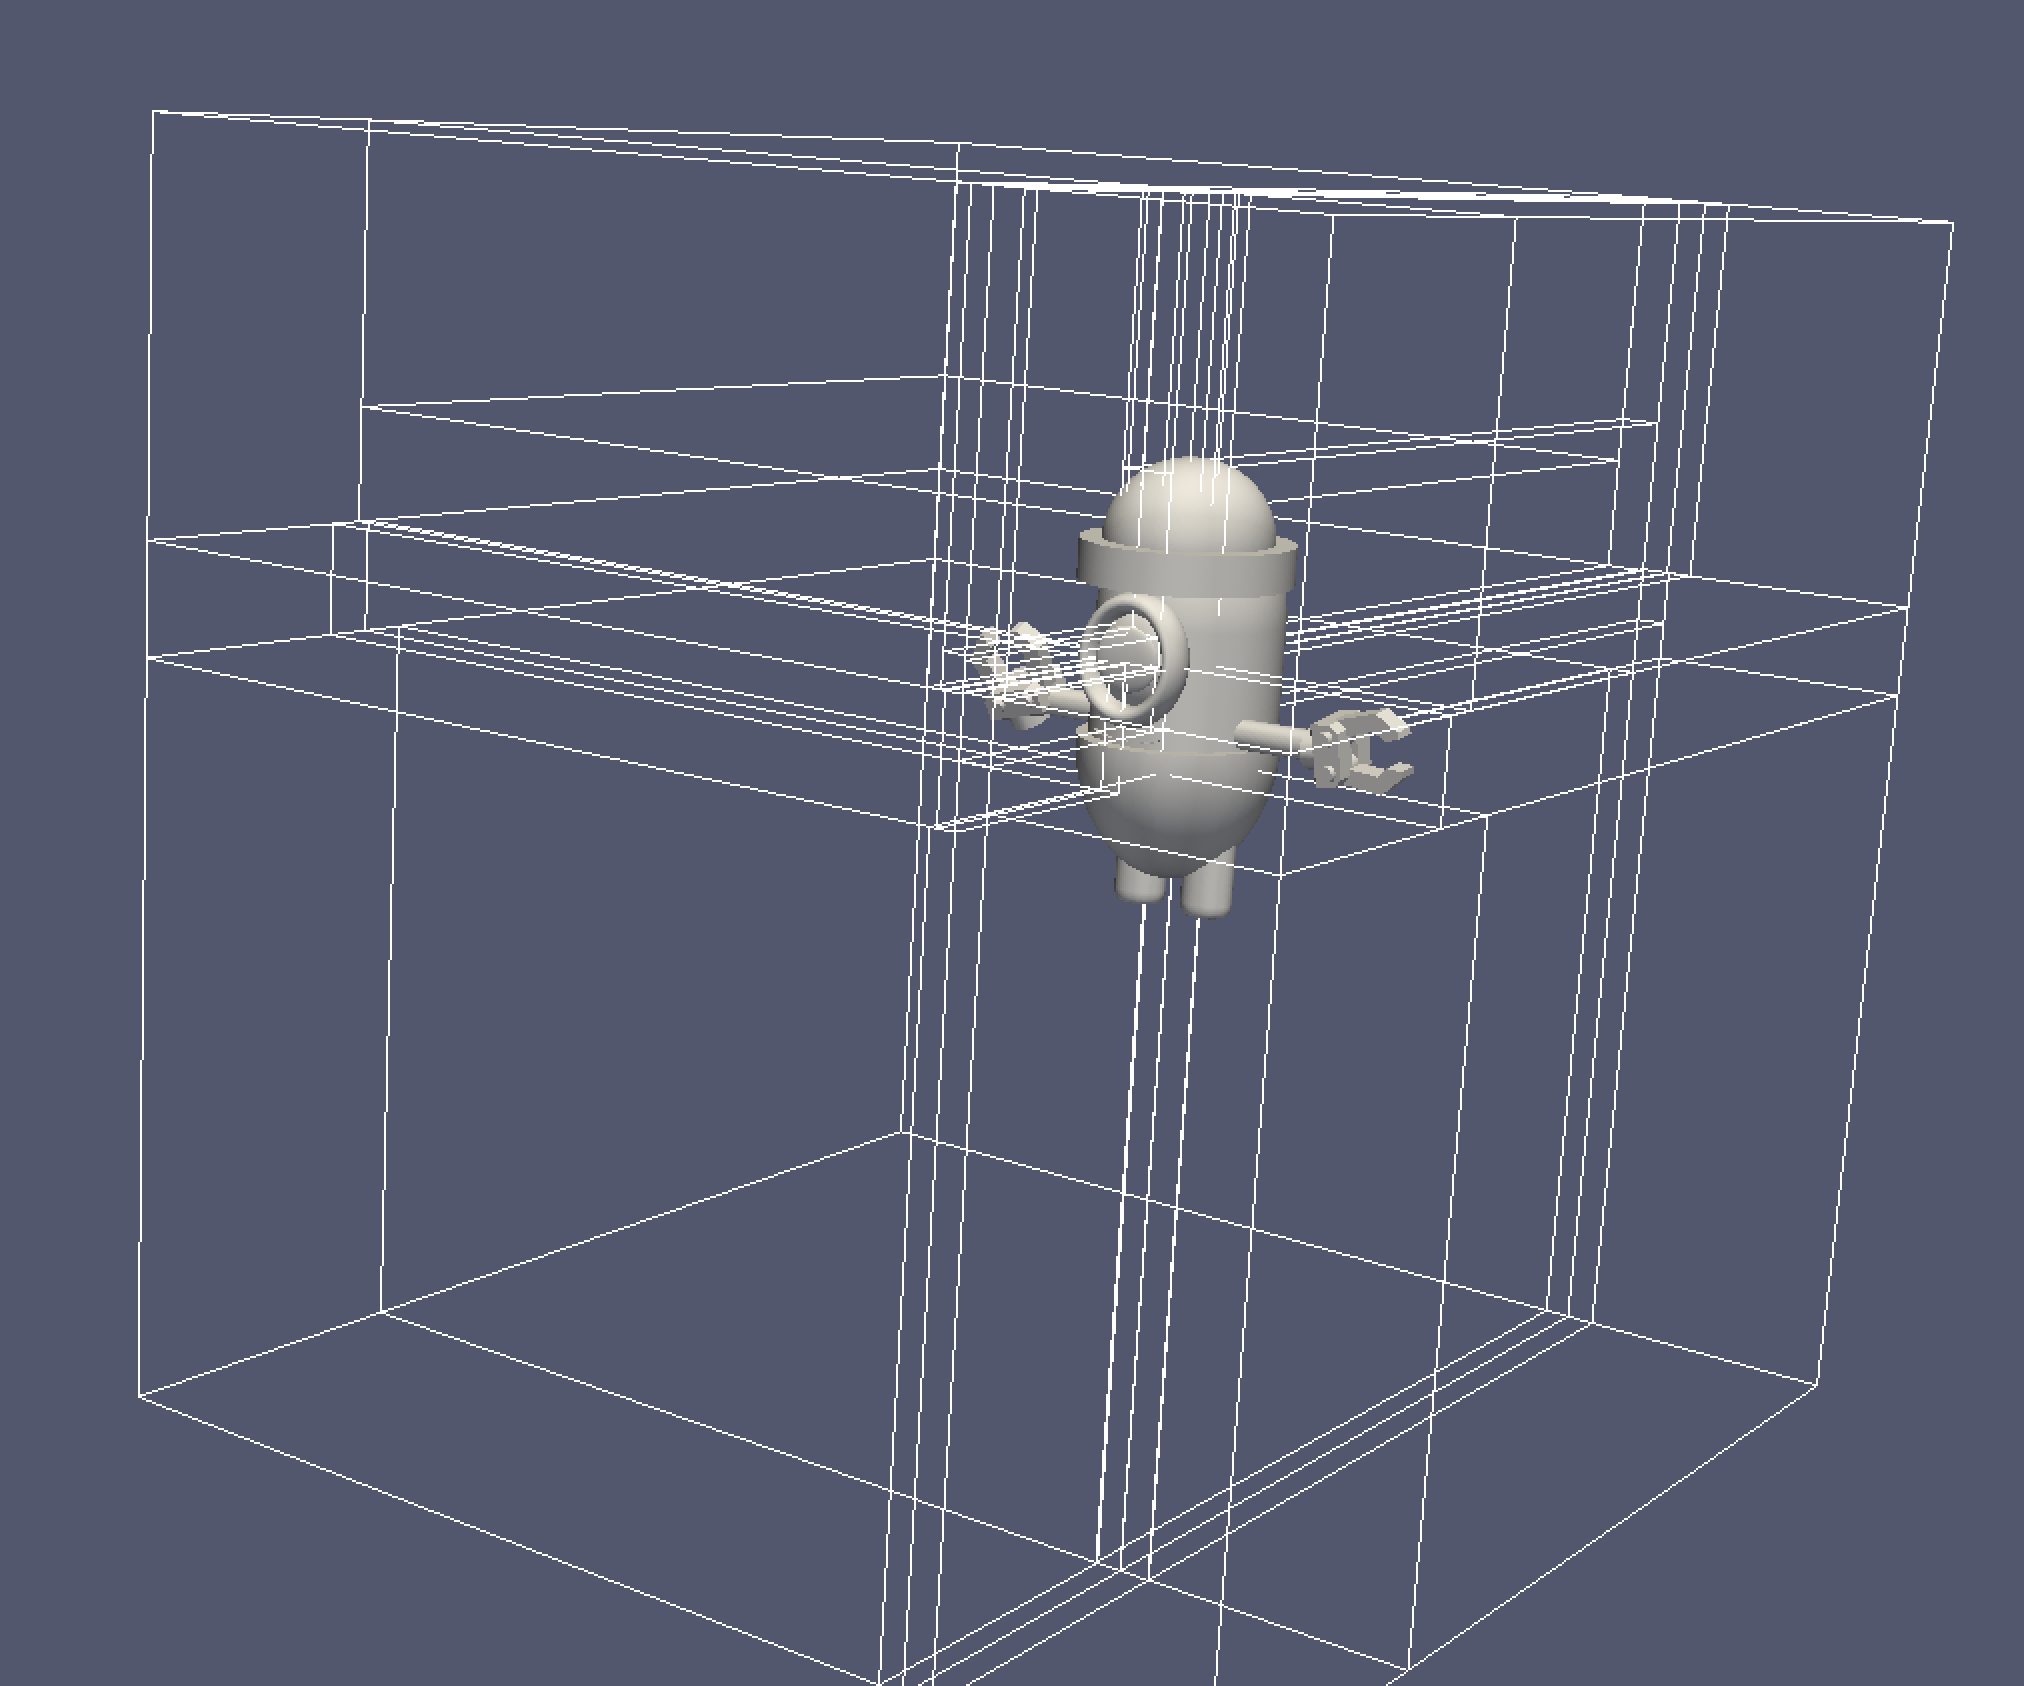
\includegraphics[width=1\textwidth]{minion} \protect\caption{\label{fig5}Spatial domain decomposition using triangular elements on 32 MPI processes, visible boundaries cut space/domain of each process.}
\end{figure}

Spatial decomposition implicitly creates logical boundaries that split space and computation (c.f. Figure \ref{fig5}). The contact detection complexity of N trianglesthat belong to $n_{i}$ particles without boundary boxes is $\sum\limits_{i=0}^n n_{i}$ = O($n^2$) in big-O notation (Algorithm \ref{alg1}). Contrary, with equally spaced boundary boxes/cells, if C is the maximum number of particles then there are $26$ neighboring cells and $max(n_{i})$ is the maximum number of triangles per particle i which result to $n_{1} \times 26 \times C \times max(n_{i})$ triangles per particle i in the local cell neighborhood. For all N triangles in the domain there are $N \times 26 \times C \times max(n_{i})$ per neighborhood. Boundary boxes due to spatial decomposition reduce the overall computational complexity to $O(n)$. Similarly, in MD simulations a cut-off range set the range of interaction fields per particle to remove redundant computation. Equally spaced boundary boxes rely on octree-based variants data structures that are great for recursive eight cell space subdivision. Our decomposition relies on non-uniform recursive subdivisions that rely on kd-tree-based data structure decomposition \cite{Brown2015} (i.e. RCB) and the number of neighbours can be arbitrarily many as they are not equally spaced, but they are equally vertex-sized. 

The number of neighbours for both methods may have an implication on communication patterns between processes. It is an open question what are the performance implications on uniform spaced octree-based decomposition versus the non-uniform kd-tree based decomposition. It is an area of investigation since on an octree-based approach information about the level of refinement is known a priori by the sub-domain boundary size, which is an interesting application for multiscale simulations. 

When spatial decomposition finishes we migrate the data to the processors (Algorithm \ref{alg7} line 2) with blocking synchronous communication. At each time step the triangles migrate according to the DEM kinematics. In addition to migration, a local area data exchange is required to communicate the boundaries of the sub-domains that cut triangles at the boundary. 

\subsection{Ghost Data Exchange}

The triangles that overlap into a remote sub-domain due to the decomposition cuts are temporary copied to one or more sub-domains in order to perform a complete contact detection. In this section, we study MPI communication characteristics when we resolve data dependencies between the sub-domains caused by ghost triangles in order to maximize performance of distributed contact detection. We explore the implication of inter-process communication and local computational performance using two communication strategies that use asynchronous non-blocking communication.

\begin{algorithm}
1. Load balance triangles

2. Migrate triangles to MPI network using blocking communication

3. Initiate neighbourhood all-to-all asynchronous MPI send/receive

4. Wait for neighbourhood asynchronous communication to terminate

5. Contact detection 

6. Derive contact forces from contact points generated

7. Explicit time integration

\protect\caption{\label{alg7}Naive Asynchronous Data Exchange Pseudocode}
\end{algorithm}

The first strategy exchanges local data to all neighbours (Algorithm \ref{alg7} line 3).  The goal is to utilize the communication bandwidth while minimise communication administration
overhead. If the exchange does not reach the upper bandwidth limit then exchange of all data is faster than filtering out the ghost triangles, i.e. doing any preprocessing that finds out which triangle from a sub-domain might be required from a neighbour. Alternatively, we can send out only triangles
that overlap from one sub-domain into another sub-domain. This filtering of triangles is an $O(N)$ operation. As soon as MPI communication finishes, the algorithm invokes the existing contact
detection routines exploiting vectorised floating point operations with a single contact detection routine. Exchange of all local data to all neighbours significantly increases the number of triangles to be processed from $T_{local}$ to $(T_{local} * N_{ranks} * T_{remote})$ where $N_{ranks}$ is the number of neighbours of neighbours. The increase of triangles to be checked increases the total computation performed locally because of the redundant triangles.

The disadvantage of such a naive method is that total MPI wait (figure \ref{fig6}) for an all-to-all neighbour data exchange increases with the number of processes. The asynchronous communication wait time results to time wasted with idle processors. The method is potentially useful with decomposition schemes where all data exchange can be processed in the background, i.e. enough bandwidth is available.

\begin{figure}[!h]
\centering
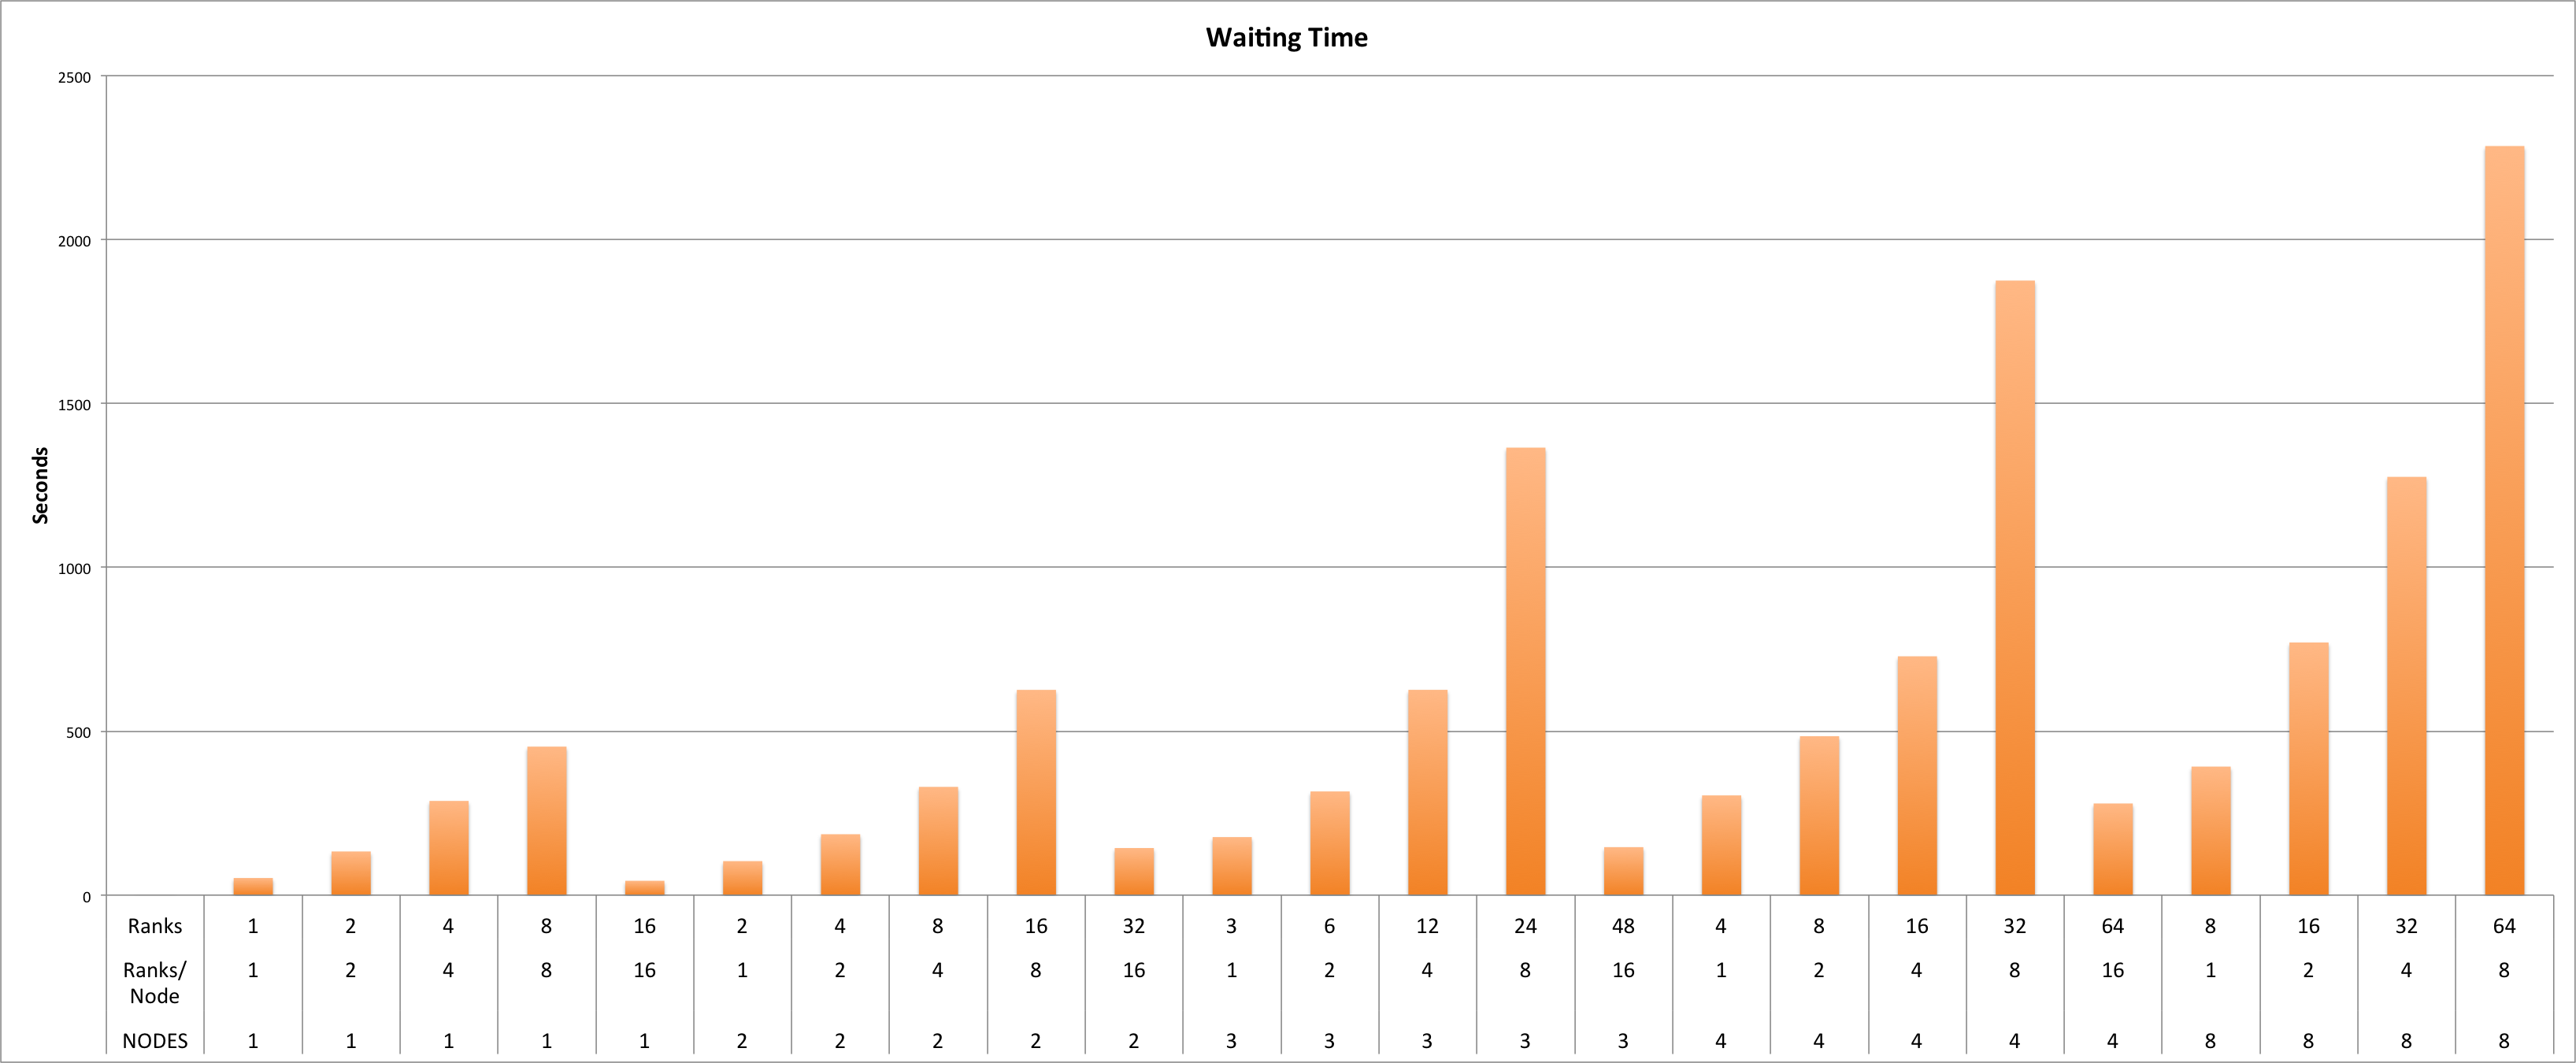
\includegraphics[width=1\textwidth]{wait} \protect\caption{\label{fig6}Waiting time (s) per MPI rank/node for all to all neighbour data exchange over 1000 time steps (25 mil triangles, 10k non-spherical particles).}
\end{figure}

\begin{algorithm}
1 Load balance triangles

2 Migrate triangles to MPI network using blocking communication

3 Search overlapping ghost triangles to send

4 Initiate neighbours asynchronous MPI send/receive

5 ~~~~~~Local contact detection

6 ~~~~~~Retrieve required ghost triangles from neighbours

7 ~~~~~~Local against to remote ghost triangle contact detection

8 Wait for neighbourhood asynchronous communication to terminate (No Real Wait)

9 Derive contact forces from contact points generated

10 Explicit time integration

\protect\caption{\label{alg8}Overlapping Asynchronous Data Exchange Pseudocode}
\end{algorithm}

The second strategy filters out local ghosts from the data structure and sends them to the overlapping neighbouring processes. Using the spatial decomposition information, we find the specific processes/boundary cells that the triangle bounding box overlaps. In this strategy we minimize data exchange at the cost of a filtering overhead and the allocation of buffers in memory. The method aims to minimise the waiting time of MPI processes by overlapping concurrent computation over communication. As shown in Algorithm \ref{alg8} line 5 local contact detection is executed as soon asynchronous MPI communication is initiated overlapping communication. A second contact detection is initiated to determine contact between local and remote ghost triangles at line 7. The strategy is advantageous as neighbour waiting is always zero as long as local contact detection takes longer than the transmission of the data. As shown in Figure \ref{fig6} the waiting time is increased proportionally to the number of MPI ranks, enabling us to increase overlapping computation per process with larger number of processes.

\begin{figure}[!h]
\centering
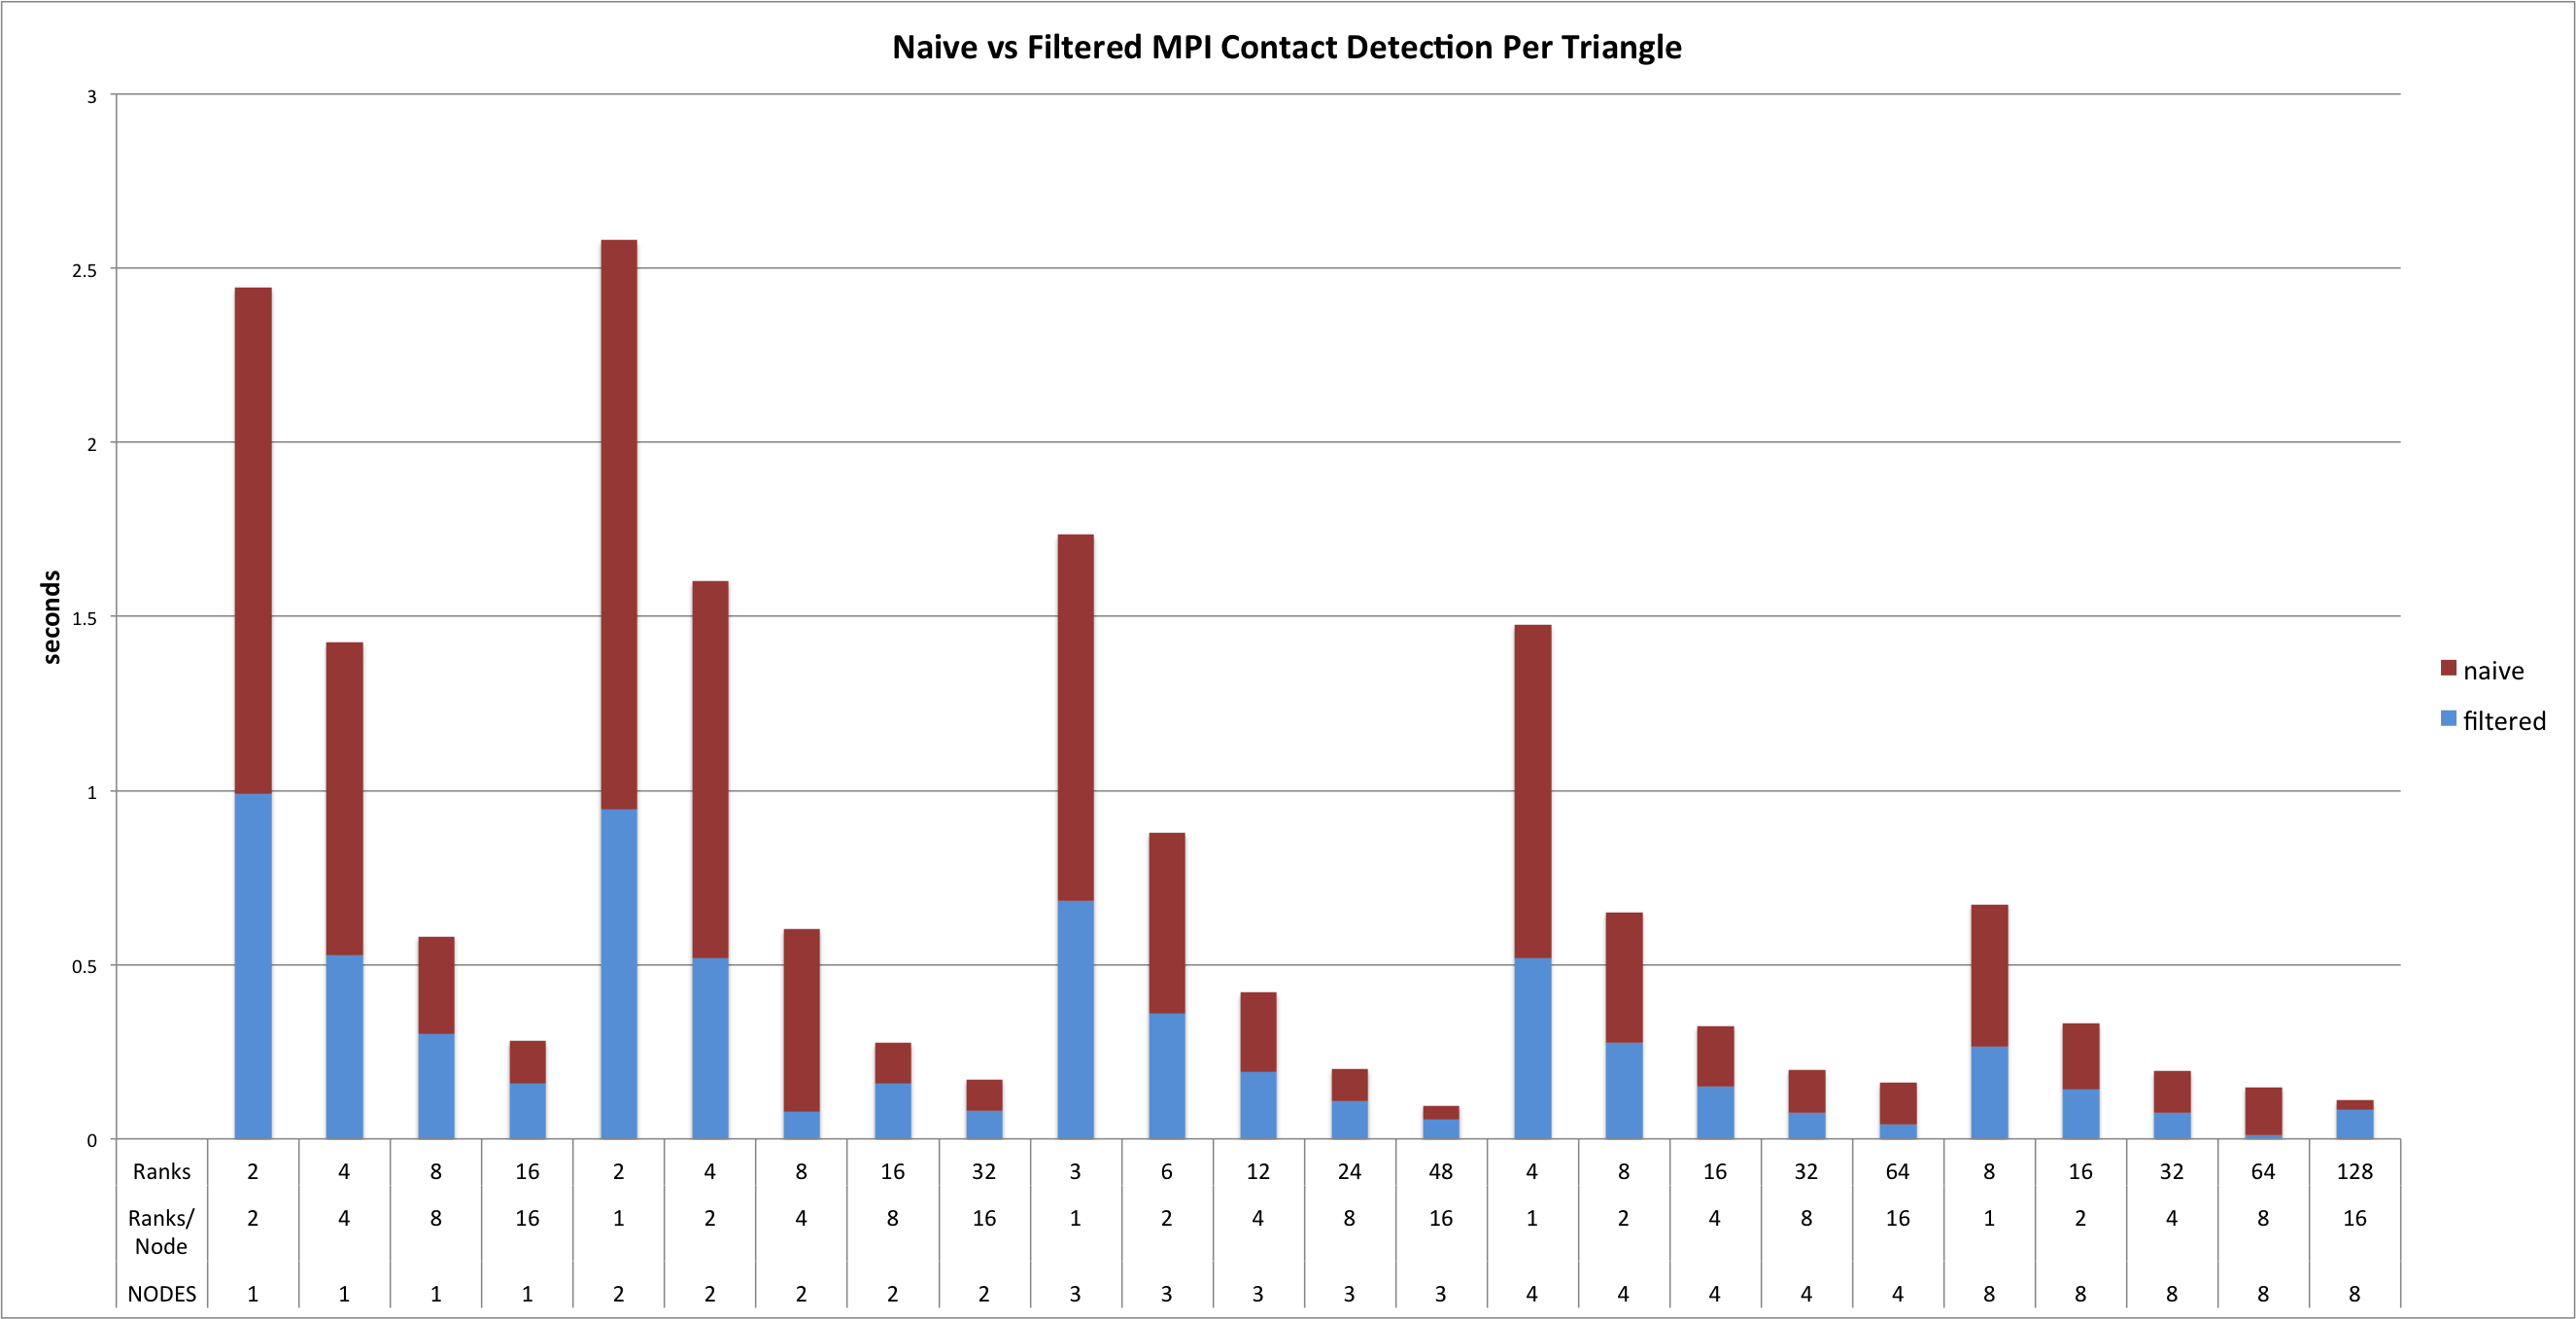
\includegraphics[width=1\textwidth]{mpi} \protect\caption{\label{fig7}Normalized naive vs filtered contact detection performance per triangle pair running on multiple nodes.}
\end{figure}

We measure both strategies to determine the performance of normalised computation per triangle. The result in Figure \ref{fig7} shows for each rank and compute node on the x axis, the time required to solve the distance of a pair of triangles. The blue bars show the average normalised time for the second strategy to process a triangle (filtering approach). The red bars show the difference between the overall naive communication time and the filtered method. The time is reduced linearly as the number of ranks increase.

For the measurement set-up in Figures \ref{fig6} and \ref{fig7}, we use Durham University Hamilton supercomputer that has per node 2 x Intel Xeon E5-2650 v2 (Ivy Bridge) 8 cores, 2.6 GHz processors, 64 GB DDR3 memory, 1 x TrueScale 4 x QDR single-port InfiniBand interconnect. 

\section{Conclusion and Future Work}

We implement a new fast but also robust hybrid algorithm that exploits modern CPU architectures. In addition, we study different schemes of domain decomposition in literature. I implement the state-of-the-art spatial domain decomposition and load balancing using Zoltan. Manual migration has been implemented using blocking MPI communication. We implement an asynchronous communication for data exchange of ghost data and compare two possible strategies. Finally based on benchmark measurements we pick the best performing scheme that overlaps computation, increases performance and decreases data exchange volume.

The next stage of my research is to investigate contact detection strategies for large scale supercomputing on a multiscale setting using adaptive multiscale grids. I'm also interested in vectorized memory layout implications on MPI buffered communication. Lastly, the source code will be generalized to form a open source library that any simulation tool can use. 

According to the project plan of the previous report, the work packages have been completed as projected.
 
\subsection{Acknowledgments}
This work has been sponsored by EPSRC (Engineering and Physical Sciences Research Council) and EDF Energy as part of an ICASE studentship. This work also made use of the facilities of N8 HPC provided and funded by the N8 consortium and EPSRC (Grant No. N8HPC{\_}DUR{\_}TW{\_}PEANO). The Centre is co-ordinated by the Universities of Leeds and Manchester. We also thank University of Durham for the supercomputing resources and technical assistance. All underlying software is open source and available at: https://github.com/KonstantinosKr/delta.

\subsection{Work Packages}

WP 1. MPI force data exchange
\begin{itemize}
\item Benchmark force per particle accumulation for DEM simulation. When contacts are determined and forces derived, the forces are required to be communicated back the ranks that hold the center of mass to update the kinematics.
\item Risk: Benchmarking and testing may take longer than March 2016.
\end{itemize}

WP 2. Total contact MPI Benchmark and code optimisation
\begin{itemize}
\item Further code optimisation for memory alignment and reducing cache misses benchmark on the total DEM code.
\end{itemize}

WP 3. Write journal paper on contact detection
\begin{itemize}
\item Report on contact detection work done over the last two years and produce a complete paper with the new insights.
\item Risk: there is a possibility that the paper writing will delay research in the next two working packages.
\end{itemize}

WP 4. Create generic and accessible library (EDF Energy, Peano, Others)
\begin{itemize}
\item Create an open source modular library so that it is usable by others in industry and in science.
\item Risk: spending more than enough time to do unnecessary non-scientific software engineering work. (eg. data input, visualization)
\end{itemize}

WP 5. Multiscale peano integration
\begin{itemize}
\item Integrate with the contact detection library into Peano framework. The goal is to use adaptive grid to create a multiscale DEM code.
\item Risk: potentially setting up the contact detection library to be usable by the framework may lead to the creation of code that is application specific instead of generic. 
\end{itemize}

WP 6. Write paper and journal on multiscaling
\begin{itemize}
\item Report on the new experiments with multiscale contact detection using the peano framework.
\item Risk: getting new results from experiments on time to produce high quality paper on time. It is a risk that is linked the implementation time required.
\end{itemize}
\cite{Tian}

\subsection{Conferences}
-Conference - Euro Par
\begin{itemize}
\item Autumn 2016
\item Conference paper on DEM with load balancing. Link: http://www.europar2015.org/
\end{itemize}

-Conference - ACME 2017
\begin{itemize}
\item Spring 2017
\item Complete code framework for large scale DEM simulations. Link: http://www.europar2015.org/
\end{itemize}

-Conference - International Supercomputing Conference
\begin{itemize}
\item May 2017
\item Whole project research. Link: http://www.isc-events.com/isc14/
\end{itemize}

\begin{sidewaysfigure}[!h]
\centering
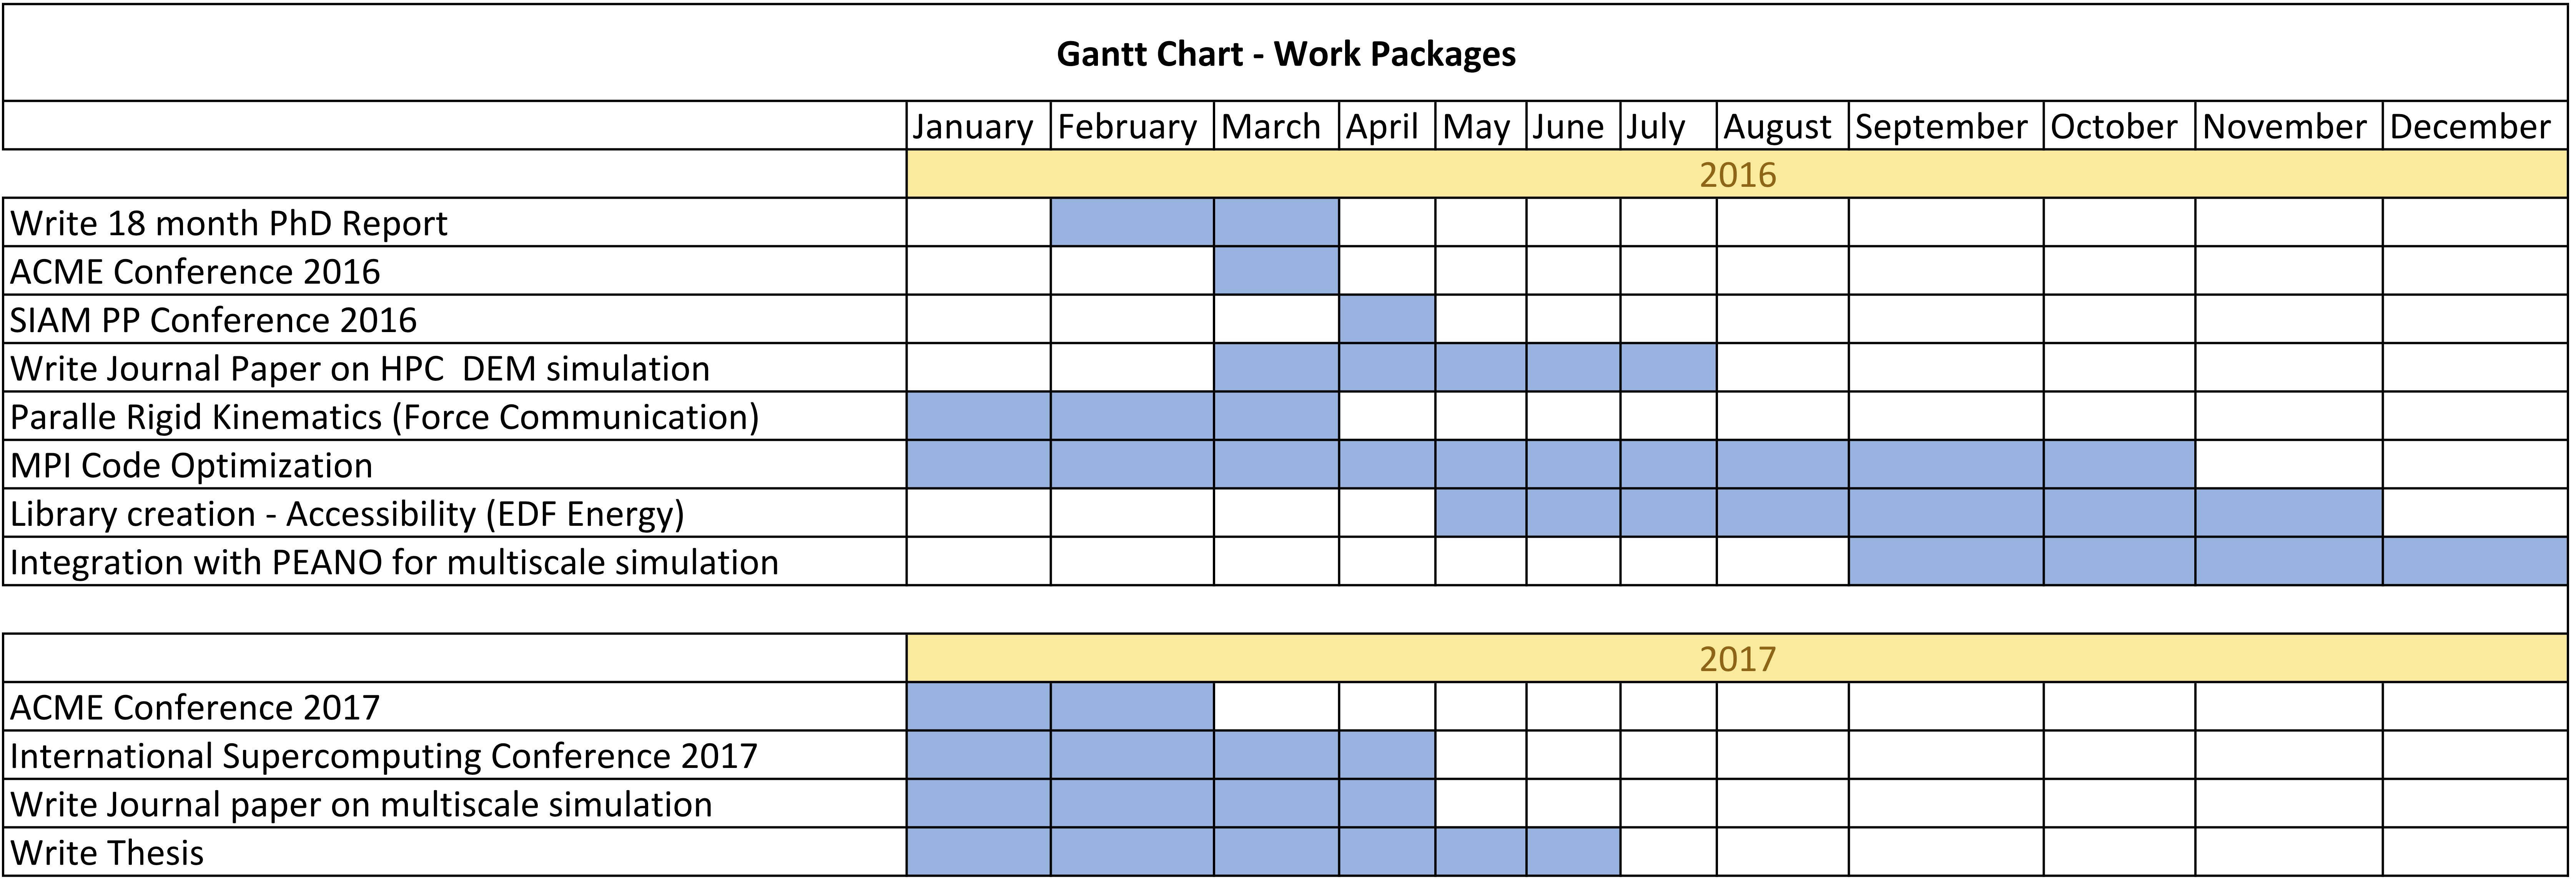
\includegraphics[width=1\textwidth]{chart} \protect\caption{\label{fig8}Timeline of Project}
\end{sidewaysfigure}  

\clearpage
\nocite{*}
\bibliography{papers}{}
\bibliographystyle{plain}


\end{document}







